\documentclass[12pt]{article}
\usepackage{amssymb}
\usepackage{nicefrac}
\usepackage{amsmath}
\usepackage{mathtools}
\usepackage[utf8]{inputenc}
\usepackage{hyperref}
\usepackage{comment}
\usepackage{pgfplots}
% \usepackage{polski}
\usepackage{parallel,enumitem}
\usepackage{mathrsfs}
\usepackage{environ}
\usepackage{dsfont}
\usepackage{geometry}
\usepackage{amsthm}
\usepackage{mdframed}
\usepackage{enumitem}
\usepackage{csquotes}
\usepackage{float}
\geometry{a4paper, portrait, margin=1in}


% \usepackage[breaklinks=true]{hyperref}

\setlength\parindent{0pt}

\DeclarePairedDelimiter\abs{\lvert}{\rvert}%
\DeclarePairedDelimiter\norm{\lVert}{\rVert}%
\DeclarePairedDelimiter\floor{\lfloor}{\rfloor}
\DeclarePairedDelimiter\ceil{\lceil}{\rceil}

% \DeclarePairedDelimiter\Pro{\lvert}{\rvert}%

% Swap the definition of \abs* and \norm*, so that \abs
% and \norm resizes the size of the brackets, and the 
% starred version does not.
\makeatletter
\let\oldabs\abs
\def\abs{\@ifstar{\oldabs}{\oldabs*}}
%
\let\oldnorm\norm
\def\norm{\@ifstar{\oldnorm}{\oldnorm*}}
\makeatother

\newcommand{\opsi}{\nicefrac{1}{\psi}}
\newcommand{\Pro}{\mathbb{P}}
\newcommand{\converges}{\xrightarrow{n \rightarrow \infty}}
\newcommand{\convergesD}{\xrightarrow[d]{n \rightarrow \infty}}
\newcommand{\env}{\mathcal{A}}
\newcommand{\Cov}{\mathrm{Cov}}
\newcommand{\corr}{\mathrm{corr}}
\newcommand{\pH}{\mathscr{H}}
\newcommand{\bH}{\mathscr{B}(\mathscr{H})}
\newcommand{\gH}{\mathscr{G}(\mathscr{H})}
\newcommand{\complex}{\mathbb{C}}
\newcommand{\real}{\mathbb{R}}
\newcommand*\Proo[1]{\Pro \left( #1 \right) }
\newcommand*\minn[1]{\min \{ #1 \} }
\newcommand*\maxx[1]{\max \{ #1 \} }
\newcommand*\conj[1]{\overline{#1}}
\newcommand*\dotprod[2]{\langle #1 , #2 \rangle}
\newcommand{\environ} {\alpha = \{ \alpha_n \}_{n\in \mathbb{Z} }}
\newtheorem{theorem}{Theorem}[section]
\newtheorem*{theorem*}{Theorem}
\newtheorem{corollary}{Corollary}[theorem]
\newtheorem{lemma}[theorem]{Lemma}
\newtheorem{fact}[theorem]{Fact}
\newtheorem{definition}[theorem]{Def.}
\newtheorem{example}[theorem]{Ex.}
\newcommand{\pder}[2][]{\frac{\partial#1}{\partial#2}}
\newcommand*{\distreq}{\stackrel{\text{d}}{=}}
\newenvironment{ftheorem}
  {\begin{mdframed}\begin{theorem}}
  {\end{theorem}\end{mdframed}}
  \newenvironment*{ftheorem*}
  {\begin{mdframed}\begin{theorem*}}
  {\end{theorem*}\end{mdframed}}
% Command for partial derivatives. The first argument denotes the function and the second argument denotes the variable with respect to which the derivative is taken. The optional argument denotes the order of differentiation. The style (text style/display style) is determined automatically
\providecommand{\pd}[3][]{\ensuremath{
\ifinner
\tfrac{\partial{^{#1}}#2}{\partial{#3^{#1}}}
\else
\dfrac{\partial{^{#1}}#2}{\partial{#3^{#1}}}
\fi
}}
\newcommand{\expect}{\operatorname{\mathbb{E}}\expectarg}
\DeclarePairedDelimiterX{\expectarg}[1]{[}{]}{%
  \ifnum\currentgrouptype=16 \else\begingroup\fi
  \activatebar#1
  \ifnum\currentgrouptype=16 \else\endgroup\fi
}

\newcommand{\innermid}{\nonscript\;\delimsize\vert\nonscript\;}
\newcommand{\activatebar}{%
  \begingroup\lccode`\~=`\|
  \lowercase{\endgroup\let~}\innermid 
  \mathcode`|=\string"8000
}


\begin{document}

\newpage
\thispagestyle{empty}
\begin{center}
\textbf{\large Uniwersytet Wrocławski\\
Wydział Matematyki i Informatyki\\
Instytut Matematyczny}\\
% \textit{\large specjalność: aktuarialno-finansowa}\\
\vspace{4cm}
\textbf{\textit{\large Wojciech Michał Fica}\\
\vspace{0.5cm}
{\Large On the favourite points of a random walk in a random environment}}\\
\end{center}
\vspace{3cm}
{\large \hspace*{5.5cm}Praca magisterska\\
\hspace*{5.5cm}napisana pod kierunkiem\\
\hspace*{5.5cm}prof. dr hab. Dariusza Buraczewskiego }\\
\vfill
\begin{center}
{\large Wrocław 2021}\\
\end{center}



% \maketitle
\pagebreak
\tableofcontents
\pagebreak
\newpage

%%%%%%%%%%%%%%%%%%%%%%%%%%%%%%%%%%%%%%%%%%%%%%%%%%%%%%%%%%%%%%%%%%%%%%%%%%%%%%%%
\section{Introduction}

Random walk is a well-known model that has been extensively studied and applied in various fields. It is a stochastic process that describes a path of a particle which moves in some fixed medium. For example, it can be used to characterise diffusion of a dye in water or virus spread during a pandemic, see \cite{COVID} or \cite{INTRO}. However, many practical applications require the environment where the system evolves to be irregular with inconsistent variations. It is natural to model such a medium as a 'random environment' where parameters for a walk are chosen at random according to some probability distribution. Surprisingly, many theorems describing walks in a random environment differ substantially from the corresponding theorems for walks in a fixed environment. This rule of thumb applies also to the main result of this article - Theorem \ref{thm:AIM}. It provides a limiting distribution of the number of visits to the most frequently visited points by a random walk in a random environment. The result is significantly different from the previously known theorem regarding walks in a fixed environment. 

\textbf{MSC classes}:	primary: 60G50, 60J80; secondary: 60F05.

%%%%%%%%%%%%%%%%%%%%%%%%%%%%%%%%%%%%%%%%%%%%%%%%%%%%%%%%%%%%%%%%%%%%%%%%%%%%%%%%
\section{Random walk in a random environment}
\subsection{General theory}
In this chapter, we provide a precise construction of a random walk in random environment (RWRE). We also fix some notation that will be used throughout the article. 

\bigskip
Firstly, we introduce a probability space that allows us to randomly choose an environment. 
\begin{equation*}
    ( \Omega, \mathcal{A}, P) = ( (0,1)^\mathbb{Z}, Bor(0,1)^\mathbb{Z}, P)
\end{equation*}
An environment is an element $ \alpha = \{ \alpha_n\}_{n \in \mathbb{Z}} $ of the measurable space  $( \Omega, \mathcal{A}).$ Once an environment $\alpha$ is chosen it remains fixed and determines transition probabilities for the walk. In this article, we consider one dimensional nearest-neighbour walks that start from the origin. 

\bigskip
Secondly, for each environment $\alpha$ there is a probability space 
\begin{equation*}
     (\Theta, \mathcal{F}, P_\alpha) = (\mathbb{Z}^\mathbb{N}, Bor(\mathbb{Z}^\mathbb{N}), P_\alpha)
\end{equation*}
where $\mathbb{Z}^\mathbb{N}$ denotes the set of all possible trajectories, $\mathcal{F}$ is the corresponding $\sigma-$algebra and $P_\alpha$ is a probability measure. A stochastic process $X = \{ X_n \}_{n \in \mathbb{N}} \in \Theta$ is a RWRE if 
\begin{equation*}
    P_\alpha ( X_0 = 0) = 1
\end{equation*}
and 
\begin{equation*}
    P_\alpha( X_{n+1} = k | X_n = l) = 
    \begin{cases} 
        \alpha_l  & \text{if} \quad k = l + 1, \\ 
        1 - \alpha_l  & \text{if} \quad  k = l - 1, \\ 
        0 & \text{otherwise.}
    \end{cases}
\end{equation*}

Finally, we introduce the ultimate probability space
\begin{equation}
    (\Omega \times \Theta, \mathcal{A} \otimes \mathcal{F}, \Pro),
\end{equation}

where $\Pro$ is a probability measure induced by letting 
\begin{equation*}
     \Pro( A \times F ) = \int_A P_\alpha(F) P(d\alpha), \quad \text{for }  A \in \mathcal{A}, F \in \mathcal{F}.
\end{equation*}

\subsection{i.i.d. environment}
For the purpose of this study we assume that the measure $P$ is chosen in such a way that $\alpha = \{ \alpha_n\}_{n \in \mathbb{Z}} $ forms a doubly infinite sequence of independent identically distributed random variables.

An extraordinary phenomenon is known for such a walk. It is possible that 
\begin{equation*}
    X_n \converges \infty \quad  \Pro \text{ a.a.} \quad \text{ and } \quad  \tfrac{X_n}{n} \converges 0 \quad \Pro \text{ a.a.}
\end{equation*}
I.e., it is possible that a walk escapes to  infinity but slower than linearly, see introductory paragraphs of \cite{KKS}. Let $m_i = \frac{1-\alpha_i}{\alpha_i}.$  The above phenomenon occurs when 
\begin{equation} \label{assumptions_v0}
    \expect{\log m_0} < 0 \quad \text{but} \quad \expect {m_0} \geq 1,
\end{equation}
see \cite{SOLOMON}. 
\bigskip

For the purpose of this article we assume that 
\begin{equation} \label{assumptions}
    \expect{\log m_0} < 0
\end{equation}
so that the walk escapes to infinity, see \cite{KKS}, but we also assume that there exists a positive number $\psi \in (0, 2)$ for which
\begin{equation}\label{eq:assump1}
    \expect{ m_0^\psi } = 1, 
\end{equation}
and 
\begin{equation}\label{eq:assump2}
    \expect{ m_0^{\psi + \delta} } < \infty \qquad  \text{ for some } \delta > 0.
\end{equation}

\subsection{Examples}
To clarify assumptions stated above, we provide a few specific examples.
\\
\textbf{Ex. 2.1.}
Firstly, note that for a walk in a fixed environment it is impossible to meet both conditions in \eqref{assumptions_v0}. Indeed, if $\alpha_0$ is a constant, and so is $m_0$, then      
$0> \expect{\log m_0} = \log m_0$ implies $1 > m_0 = \expect{m_0}.$
\\
\textbf{Ex. 2.2.}
Secondly, consider a RWRE where the environment $\environ$ is i.i.d. with distribution
\begin{equation*}
    \Pro(\alpha_0 = \nicefrac{3}{4}) = \nicefrac{3}{5} \qquad \text{and} \qquad \Pro(\alpha_0 = \nicefrac{1}{3}) = \nicefrac{2}{5}.\footnote{This is an example adapted from \cite{PETERSON}. }
\end{equation*}
Then 
\begin{equation*}
    \expect{m_0} = 1 \qquad \text{and} \qquad \expect{\log m_0} \approx -0.38 < 0.
\end{equation*}
So the conditions in \eqref{assumptions_v0} are met.
\\
\textbf{Ex. 2.3.}
Thirdly, we want to provide some intuitions why random environment allows for a convergence to infinity that is slower than linear. For a RWRE, if  $\expect{\log m_0} < 0$  then the walk drifts towards infinity. If simultaneously  $\expect{m_0} > 1$ then $\Pro(m_0 > 1) >0$. But 
\begin{equation*}
    0 < \Pro(m_0 > 1 ) = \Pro(\tfrac{1-\alpha_0}{\alpha_0} > 1) = \Pro(\alpha_0 < \tfrac{1}{2}).
\end{equation*}
Hence, the walk may experience local drifts towards $-\infty$. This causes the delay in converging to $+\infty$. The delay is measured by the parameter $\psi$. In particular, the delay leads to a sublinear convergence.
\\
\textbf{Ex. 2.4.}
Lastly, note that if we assume \eqref{assumptions_v0} with a slightly stronger condition, namely $\expect{m_0} > 1$ then there exists a unique positive $\psi \in (0,1) $ such that both \eqref{eq:assump1}
 and \eqref{eq:assump2} hold. Indeed, let $$\Lambda(s) = \expect{m_0^s}.$$ We may prove \eqref{eq:assump1}
 and \eqref{eq:assump2} easily by using the below facts
 \begin{itemize}
    \item $\Lambda(0) = 1$ and $\Lambda(1) > 1$.
    \item $\Lambda^\prime(0) = \expect{\log m_0} < 0$.
    \item $\Lambda$ is a convex function.
 \end{itemize} See Figure \ref{fig:psi}.
 
\begin{figure}[htb] 
    \centering
    \resizebox{0.6\textwidth}{!}{%
    \begin{tikzpicture}
    \begin{axis}[
        ticks = none,
        axis lines = left,
        xlabel = $s$,
        ylabel = {$\Lambda(s)$},
        % yticklabels={,,},
        % xticklabels={,,}
        xmin=0, xmax=1.3,
        ymin=0, ymax=1.8
    ]
    
    \addplot[black] (1,1.5) circle (2pt) node[anchor=west] {$\expect{m_0}$};
    \addplot[black] (0,1) circle (2pt) node[anchor=south west] {1};
    \addplot[black] (1,0) circle (2pt) node[anchor=south west] {1};
    \addplot[black, dashed] coordinates{(0,1) (0.8333,1)};
    \addplot[black, dashed] coordinates{(0.8333,0) (0.833,1)};
    \addplot[black] (0.8333,0) circle (2pt) node[anchor=south west] {$\boldsymbol{\psi}$};
    %Below the red parabola is defined
    \addplot [
        samples=300, 
        color=black,
    ]
    % {1.2*x^2 - 1.1*x + 1};
    {3*x^2 - 2.5*x + 1};
    \end{axis}
    \end{tikzpicture}
    }%
\caption{A visual depiction of the parameter $\psi$.}
\label{fig:psi}
\end{figure}

 
\section{Correspondence between random walks and branching processes}
Now, we briefly introduce a well known correspondence between random walks and branching processes. The below explanation is taken from \cite{KKS}. Recall that $X_n$ is, as always, a RWRE. Define 
\begin{equation*}
\begin{aligned}
    T_n &= \min \{ t : X_t = n\} = \text{hitting time of }  \{n\}, \\
    U_i^n &= \text{number of steps from } i \text{ to } i-1 \text{ during } [0, T_n) \\
    &= \abs{ \{t < T_n : X_t = i, X_{t+1} = i-1 \} }.
\end{aligned}
\end{equation*}
Observe, that 
\begin{equation*}
\begin{aligned}
    n &= X_{T_n} - X_0 \\
     &= \text{number of steps to the right during } [0, T_n) -  \text{number of steps to the left during } [0, T_n).
\end{aligned}
\end{equation*}
Hence
\begin{equation*}
\begin{aligned}
    T_n &= \text{number of steps during } [0, T_n) \\
     &= \text{number of steps to the right during } [0, T_n) +  \text{number of steps to the left during } [0, T_n) \\ 
     &= n + 2 \times  \text{number of steps to the left during } [0, T_n) \\
     &= n + 2 \sum_i U_i^n.
\end{aligned}
\end{equation*}

By the definition of $U_n^i$, $U_n^i = 0$ for  $i \geq n$ and
\begin{equation*}
    \sum_{i \leq 0} U_i^n \leq \text{ total time spent by } X_t \text{ in } (-\infty, 0] < \infty \quad \Pro \text{ a.a. }
\end{equation*}
because $X_t \converges \infty \quad \Pro $ a.a. under  \eqref{assumptions}. Hence we are mostly interested in $U_i^n$ for $i \in \{1 \dots n -1\}.$ 
\bigskip

Now we discover a branching process hidden in the process $X_t$. We start by describing how to transform a trajectory of a RWRE into a forest (a list of trees representing a branching process) and then we provide a formal construction. 
\bigskip

Figure \ref{fig:walk} depicts a trajectory of a RWRE. Green segments represent moves to the right and red segments represent moves to the left. Dotted points mark the first visits on a given positive level. Figure \ref{fig:gw} depicts the corresponding branching process. Transformation of Figure \ref{fig:walk} into Figure \ref{fig:gw} is illustrated in Figure \ref{fig:walk_merging} and can be done as follows
\begin{itemize}
    \item remove all green segments whose right end is a dotted point;
    \item apply glue from above on all the remaining segments;
    \item fold the plot horizontally so that corresponding segments will be glued together. 
\end{itemize}

\bigskip

Now, we provide a formal construction. For a moment fix the environment $\environ$. Conditionally on this environment $X_t$ is a Markov chain. A step from $i$ to $i-1$ can happen 
\begin{itemize}
    \item either between $T_i$ and the first step from $i$ to $i+1,$
    \item or between two successive steps from $i$ to $i+1.$
\end{itemize}
When $X_{t_0} = i$ for some $t_0$, then the conditional probability, given $\environ$ and $X_0, \dots , X_{t_0}$ of going $k$ times from $i$ to $i-1$ before the next move from $i$ to $i+1$ is $\alpha_i(1-\alpha_i)^k.$ From this we see that the conditional distribution of $U_i^n$, given $\env$ and $U_{i+1}^n, \dots, U_{n-1}^n$ is precisely the distribution of the sum of $1 + U_{i+1}^n$  independent random variables $V_1, V_2, \dots$, each with geometric distribution 
\begin{equation}\label{e:offspring_distr}
    P_\alpha(V_l = k) = \alpha_i(1-\alpha_i)^k.
\end{equation}
In other words, for a fixed $\environ$ and $n$ the sequence $U_n^n = 0, U_{n-1}^n, \dots, U_1^n$ has the distribution of the first $n$ generations of an inhomogeneous branching process with one immigrant in each generation and with offspring distribution  \eqref{e:offspring_distr} for all particles in the $(n-i-1)^\text{th}$ generation. When $\environ$ is random then the branching process also evolves in random environment. The book \textit{Branching processes}, \cite{BRANCHING}, elaborates very diligently on these matters. Because $\alpha_{n-1}, \dots, \alpha_0$ have the same distribution as $\alpha_0, \dots, \alpha_{n-1}$ it follows that the sequence $U_n^n = 0, U_{n-1}^n, \dots, U_1^n$ has the same distribution as $Z_0, \dots, Z_{n-1}$ where $Z_0 = 0, Z_1 , Z_2, \dots$ forms a branching process in random environment with one immigrant each unit of time and offspring distribution \eqref{e:offspring_distr}. 

\begin{figure}[H]
    \centering
    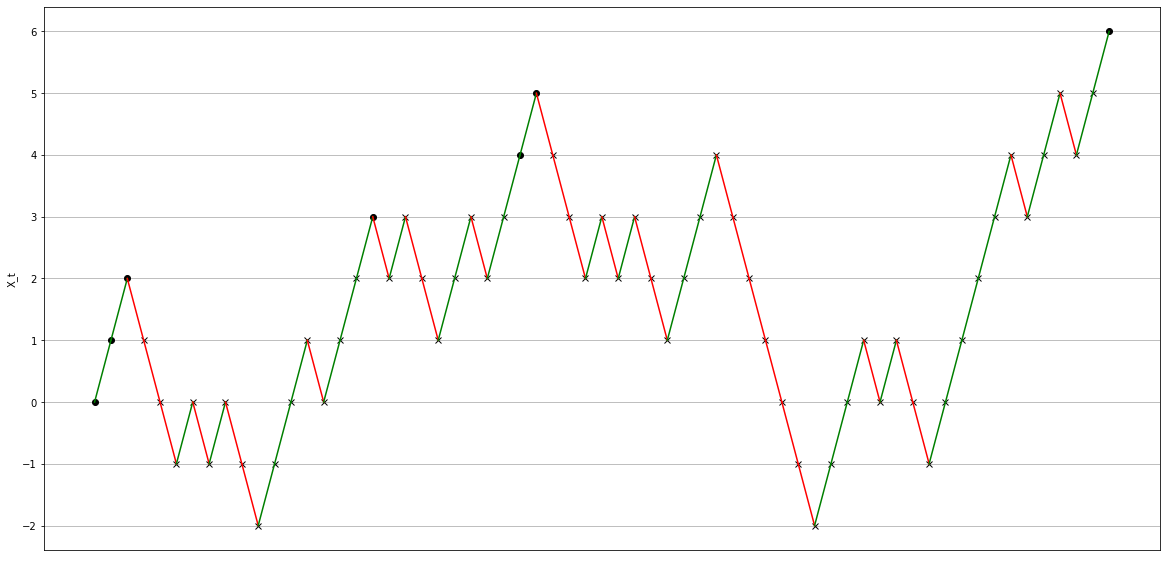
\includegraphics[width=\textwidth,height=\textheight,keepaspectratio]{walk.png}
    \caption{A realization of a RWRE until time $T_6$, i.e. until the walk $X_t$ reaches level 6. Dotted points represent the first visits on a given positive level. For example, $U_4^6 = 3$ or $U_3^6 = 7$.}
    \label{fig:walk}
\end{figure}

\begin{figure}[H]
    \centering
    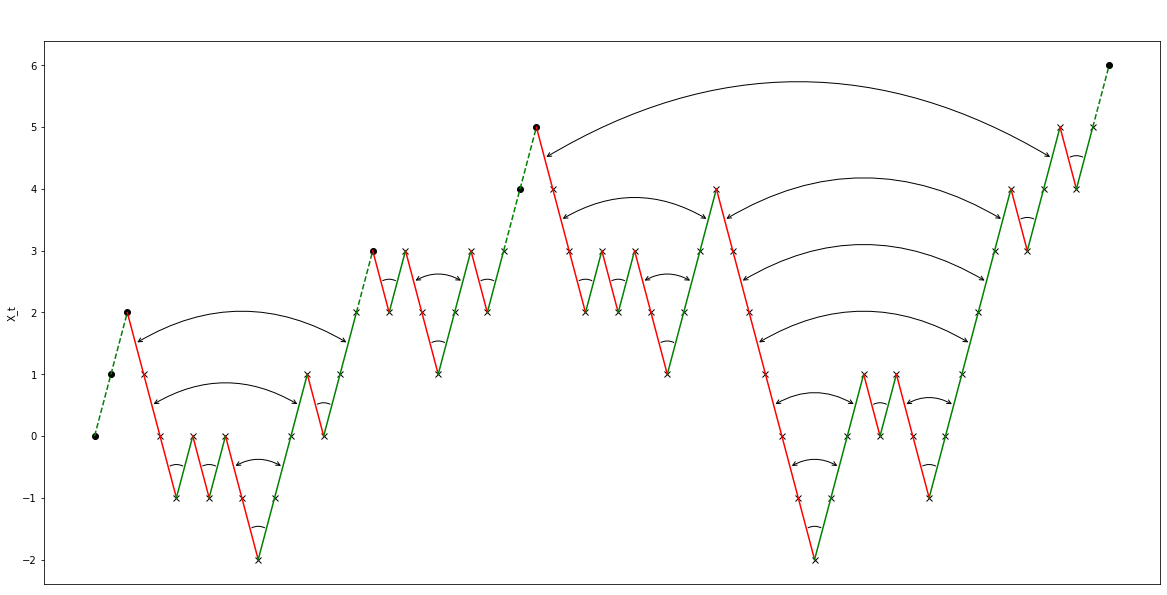
\includegraphics[width=\textwidth,height=\textheight,keepaspectratio]{walk_merging.png}
    \caption{Transformation of a trajectory of a RWRE into a realisation of a branching process. Dashed green lines are removed, segments pointed by arcs are glued together.}
    \label{fig:walk_merging}
\end{figure}

\begin{figure}[H]
    \centering
    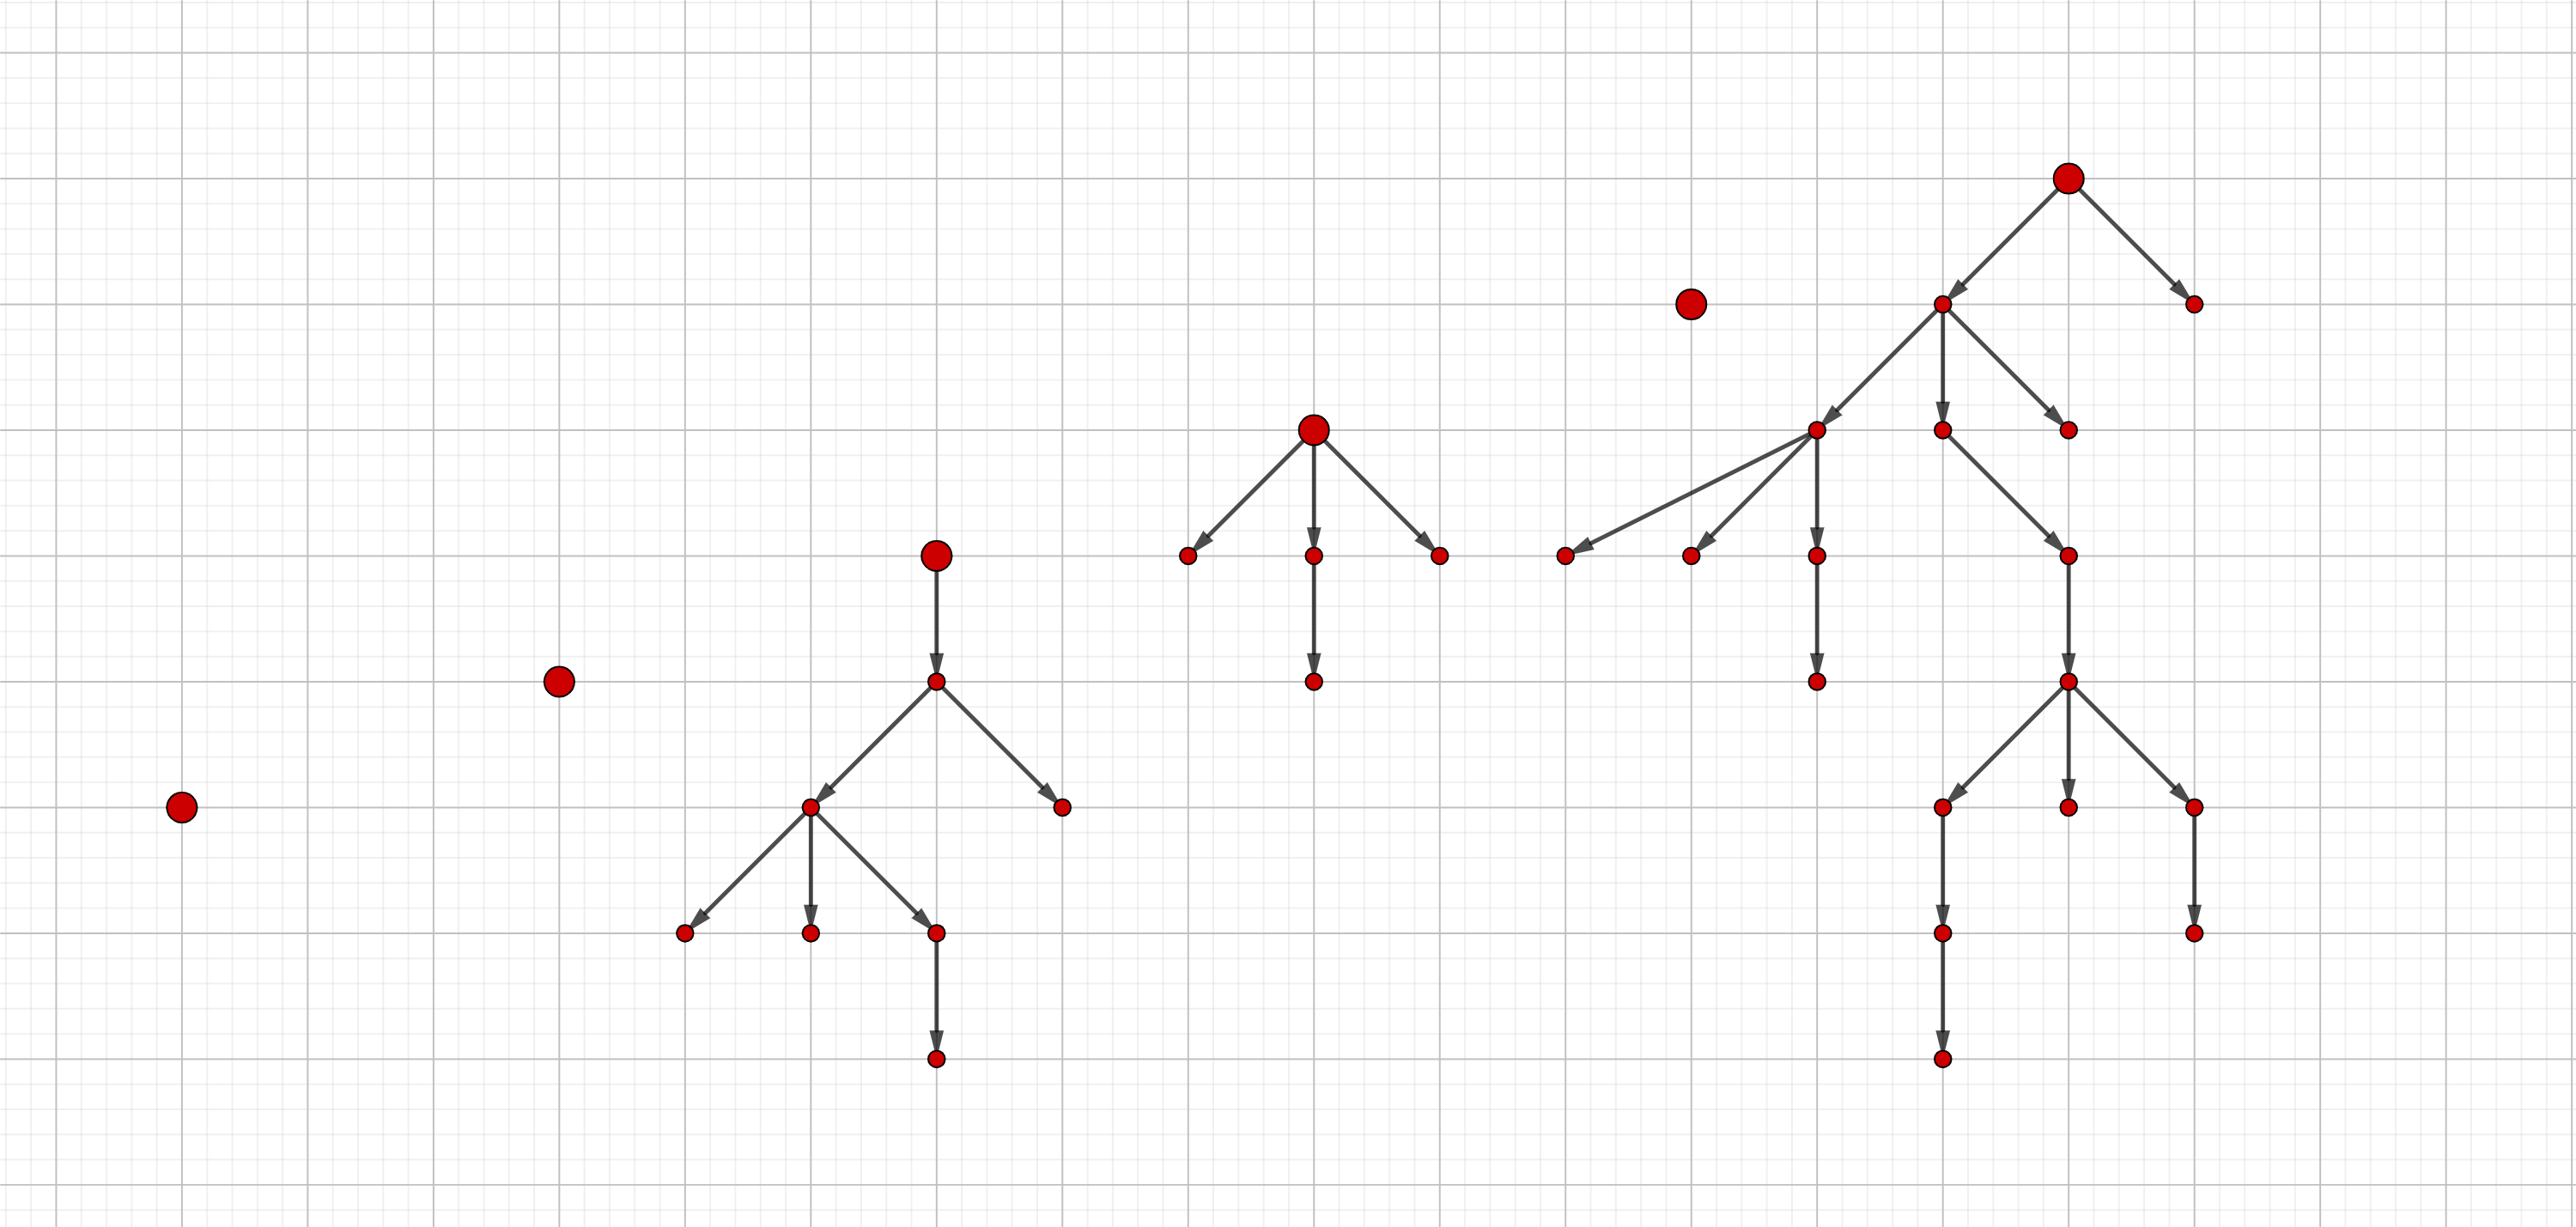
\includegraphics[width=\textwidth,height=\textheight,keepaspectratio]{GW.png}
    \caption{A branching process $Z_t$ that corresponds to the walk in figure \ref{fig:walk}. Large dots represent immigrants. Recall that we number the epochs from 0 and $\xi_{l,k}$ = number of offspring of the $k-$th particle in the $l-$th generation of the branching process $\{Z_t\}.$ Here             $\xi_{1,0} = 0$, i.e. the first particle (the immigrant) in the first epoch has no children.         $\xi_{1,1} = 3$, i.e. the second particle in the first epoch has 3 children.         $\xi_{1,2} = 0$, i.e. the third particle in the first epoch has no children.}
    \label{fig:gw}
\end{figure}


%%%%%%%%%%%%%%%%%%%%%%%%%%%%%%%%%%%%%%%%%%%%%%%%%%%%%%%%%%%%%%%%%%%%%%%%%%%%%%%%
\section{Problem answered by the article}

Let $X_n$ be a RWRE. In this paper we are interested in calculating how many times the walk visits a given point. Namely, let 
\begin{equation*}
\begin{aligned}
    \eta(x, n) &= \abs{ \{ k \leq T_n : X_k = x \}} \qquad \text{ for } x \in \mathbb{Z},  \\ 
    \eta^{*}(n) &= \sup_{x \in \mathbb{Z}} \eta(x, n).
\end{aligned}
\end{equation*}
We prove that  $\dfrac{\eta^*(n)}{n^{\nicefrac{1}{\psi}}}$ converges to the Fréchet distribution, i.e.
\begin{ftheorem}\label{thm:AIM}
Assume \eqref{assumptions}, \eqref{eq:assump1} and \eqref{eq:assump2}, then, for $y > 0$,
\begin{equation} \label{the_aim}
    \Proo{\dfrac{\eta^*(n)}{n^{\nicefrac{1}{\psi}}} > y} \converges 1 - \exp(-Cy^{-\psi})
\end{equation}    
for some constant $C$.
\end{ftheorem}

\bigskip

Note that visits on negative levels are irrelevant from the perspective of \eqref{the_aim}. Indeed, 
\begin{fact}\label{f:eta_negative}
\begin{equation} 
    \dfrac{ \sup_{x \in \mathbb{Z}, x < 0} \eta(x, n)  }{n^{\nicefrac{1}{\psi}}} \converges 0 \qquad \Pro \text{ a.a.}
\end{equation}
\end{fact}
\begin{proof}
    For $x < 0$ 
    \begin{equation*}
        \eta(x, n) \leq \text{ total time spent by the walk in } (-\infty, 0) < \infty 
    \end{equation*}
    because  $X_t \converges +\infty.$
\end{proof}

Now, observe that
\begin{equation}\label{eq:slusky}
     \dfrac{ \sup_{x \in \mathbb{Z}, 0\leq x < n} \eta(x, n)  }{n^{\nicefrac{1}{\psi}}} \leq  \dfrac{  \eta^*( n)  }{n^{\nicefrac{1}{\psi}}} \leq  \dfrac{ \sup_{x \in \mathbb{Z}, x < 0} \eta(x, n)  }{n^{\nicefrac{1}{\psi}}} +  \dfrac{ \sup_{x \in \mathbb{Z}, 0\leq x < n} \eta(x, n)  }{n^{\nicefrac{1}{\psi}}} + \dfrac{1}{n^{\nicefrac{1}{\psi}}}.
\end{equation}
Indeed, we obtain the lower bound by taking the $\sup$ over a smaller set and the upper bound by splitting the $\sup$ domain into 3 parts $\{x < 0 \}$, $\{ 0\leq x < n\}$ and $\{x = n\}$.  Fact \ref{f:eta_negative}, inequalities in \ref{eq:slusky} and Slutsky's theorem, see \cite{SLUTSKY}, imply that in order to achieve limiting distribution of $\dfrac{  \eta^*( n)  }{n^{\nicefrac{1}{\psi}}}$ it is enough to analyse the behaviour of  $\dfrac{ \sup_{x \in \mathbb{Z}, 0\leq x < n} \eta(x, n)  }{n^{\nicefrac{1}{\psi}}}$.

\bigskip

Thanks to the correspondence between RWRE and branching processes in random environment (BPRE) we can express $\eta(x, n)$ in terms of process $Z_t$, namely
\begin{lemma}\label{l:eta}
    For $ 0 \leq x  < n$ 
    \begin{equation}\label{e:eta_Z}
        \eta(x, n) \distreq 1 + Z_{n - x -1} + Z_{n-x}
    \end{equation}
\end{lemma}
\begin{proof}
$\eta(x, n)$ counts how many times the walk visited level $x$. It is equivalent to the sum of 
\begin{itemize}
    \item 1 = the first entry on level  $x$ 
    \item $Z_{n-x-1}$ = number of times the walk went from level  $x+1$  to level  $x$ 
    \item $Z_{n-x}$ =  number of times the walk went from level  $x$  to level  $x-1$.  Every time the walk enters level  $x-1$  it has to return to level $x$, because  $X_t \converges +\infty.$ 
\end{itemize}
\end{proof}

\bigskip

Looking back at \eqref{e:eta_Z}, it seems sensible to focus first on $ M_n^\prime = \max_{k=1 \dots n}Z_k$ before calculating $M_n = \max_{k=1 \dots n}(Z_k + Z_{k-1}).$ We first provide a few facts about $M_n^\prime$ and then return to $\eta^*(n).$


\section{Notation}
Let us fix some notation
\begin{enumerate}
    \item $\{ \alpha_n \}_{-\infty < n < \infty }$ - an i.i.d. sequence of random variables with values in [0,1] - \textit{the environment}. 
    \item $\env  = \sigma\{ \alpha_n : -\infty < n < \infty \}.$
    \item $m_i = \dfrac{1-\alpha_i}{\alpha_i}$ - an i.i.d. sequence. Throughout the article we assume that $\expect{\log m_0} < 0 \text{ and } \expect {m_0} \geq 1.$
    \item $\psi \in (0, 1)$ - a unique positive number for which $\expect{\left( m_0 \right)^\psi } = 1.$
    \item $Z_0 = 0, Z_1, Z_2, \dots$ - a branching process in a random environment with one immigrant in each epoch and offspring distribution as in \eqref{e:offspring_distr}. 
    \item $\xi_{l,k}$ = number of offspring of the $k-$th particle in the $l-$th generation of the branching process $\{Z_t\}.$
    \item $S_{l,k} = $ number of descendants alive in epoch $k$ of the $Z_l$ particles present at time $l$.
    \item $Y_s$ total progeny of immigrant $s$.
    \item $R_n  = \expect{Z_n | \env}.$ In a sense, as we shall see, $R_n$ behaves similarly to $Z_n$.
    \item $\nu = \inf \{n : Z_n = 0\}$ - a stopping time, an \textit{extinction} time.
    \item For a fixed $A>0$, let $\sigma = \sigma (A) = \inf \{ n : Z_n > A\}$ - a stopping time. 
\end{enumerate}
    

%%%%%%%%%%%%%%%%%%%%%%%%%%%%%%%%%%%%%%%%%%%%%%%%%%%%%%%%%%%%%%%%%%%%%%%%%%%%%%%%
\section{Stochastic recursions}

Process $Z_n$ has properties similar to those of some stochastic recursion. Now, we shall provide a few known results regarding the recursion. They are not necessary for the proof of the main theorem. But hopefully, they could help with getting some intuitions on issues considered in this paper. The proof of the main result is provided in the subsequent chapters.

\begin{fact}
    $R_n$ follows a recursive formula
    \begin{equation} \label{e:f2}
    \begin{cases}
        R_0 &= 0, \\
        R_n &= m_{n-1}R_{n-1} + m_{n-1} \qquad \text{ for } n \geq 1.
    \end{cases}
    \end{equation}
\end{fact}
\begin{proof}
Of course, $R_0 = \expect{Z_0|\env} = \expect{0|\env} = 0$. Now, we show that $R_1 = m_0$.     This is evident. Given an environment  $\environ$, $Z_1$ is a random variable distributed with geometric distribution with parameter $\alpha_0$, i.e. $Z_1(\alpha, \cdot) \sim Geo(\alpha_0)$. Moreover, $m_0$ is $\env$-measurable and for any $A \in \env$
\begin{equation} \label{e:f1}
    \int_{A \times \Theta} Z_1 d\mathbb{P} = \int_{A} \int_{\Theta} Z_1(\alpha, t) dP_\alpha(t) dP(\alpha) = \int_A \expect{Z_1(\alpha, \cdot)} dP(\alpha) = \int_A m_0 dP(\alpha) = m_0.
\end{equation} 
Now, using the same reasoning as in \eqref{e:f1}, we see that 
\begin{equation*}
    \expect{ \xi_{n-1,l} | \env, Z_{n-1} = j} = m_{n-1}, \qquad \text{ for } 0 \leq l < j.
\end{equation*}
Hence, 
\begin{equation*}
\begin{aligned}
    R_n &= \expect{Z_n|\env} = \expect{\sum_{k=0}^{Z_{n-1}} \xi_{n-1,k} |\env} = \sum_{j=0}^{\infty} \expect{\sum_{k=0}^{j} \xi_{n-1,k} | \env, Z_{n-1} = j} \Pro(Z_{n-1} = j | \env)  \\ 
    &= \sum_{j=0}^{\infty} \sum_{k=0}^{j} \expect{ \xi_{n-1,k} | \env, Z_{n-1} = j} \Pro(Z_{n-1} = j | \env) =  \sum_{j=0}^{\infty} (j+1)m_{n-1}\Pro(Z_{n-1} = j | \env)  \\
    &= \expect{(Z_{n-1} + 1)m_{n-1}|\env} = m_{n-1} \expect{Z_{n-1} +1 | \env} = m_{n-1}(R_{n-1}+1).
\end{aligned}
\end{equation*}
\end{proof}
Equation \eqref{e:f2} is an example of stochastic affine recursion. Processes like these were studied by many authors, for example see \cite{KESTEN_REC}. By lemma 1 from \cite{KKS} we know that 
\begin{lemma}\label{l:Rn_conv}
    Assume that the distribution of $m_i$ is non-arithmetic, $\expect{m_i^\psi} = 1, \expect{\log m_i} < 0 $ and  $\expect{m_i^{\psi + \delta}} < \infty $ for some $\delta > 0$.
    Then, the stochastic recursion 
    \begin{equation*}\label{e:recursion}
        \begin{cases}
            W_0 = 0 \\
            W_n = m_{n-1}W_{n-1} + m_{n-1},
        \end{cases}
    \end{equation*}
    converges in distribution, i.e.
    \begin{equation} 
        W_n \xrightarrow[d]{n\rightarrow \infty} \nu \quad \text{where} \quad  \nu(t, \infty) \sim C t^{-\psi},
    \end{equation}
    for some constant $C$. The above result is also true if the initial condition $W_0 = 0$ is replaced by $W_0 \sim \nu$.
\end{lemma}
Moreover, by lemma 3.1.4 from \cite{DBURA1} it is known that
\begin{lemma} \label{l:Q_n}
    The maxima $ Q_n = \max_{k=1 \dots n}W_k$ of a stochastic recursion 
    \begin{equation*}\label{e:recursion2}
        \begin{cases}
            W_0 \sim \nu \\
            W_n = m_{n-1}W_{n-1} + m_{n-1},
        \end{cases}
    \end{equation*}
    converge in distribution, i.e., 
    \begin{equation} \label{e:M_thilda_conv}
        \Pro(Q_n \leq n^{\nicefrac{1}{\psi}} x ) \converges \exp(-\theta x^{-\psi}),
    \end{equation}
    for some constant $\theta > 0$ and $\nu$ from Lemma \eqref{l:Rn_conv}.
\end{lemma}

We would like to apply the above lemma for the recursion $R_n$. To do so, we need to prove that the theorem holds when the initial condition $W_0 \sim \nu$ is replaced by $W_0 = 0.$

\begin{theorem} \label{th:M_tilda}
    The maxima $ \widetilde{M}_n = \max_{k=1 \dots n}R_k$ converge in distribution, namely
    \begin{equation} \label{e:M_thilda_conv}
        \Pro(\widetilde{M}_n \leq n^{\nicefrac{1}{\psi}} x ) \converges \exp(-\theta x^{-\psi}),
    \end{equation}
\end{theorem}
\begin{proof}
    This follows from Lemma \ref{l:Q_n}. Let us use the same notation as in Lemma \ref{l:Q_n}. We compare $W_n$ with $R_n$. They follow the same recursive pattern but $R_n$ starts from $R_0 = 0$.
    \begin{align*}
        \abs{W_0 - R_0} &= \abs{W_0} \\
        \abs{W_1 - R_1} &= \abs{m_0W_0 + m_0 - m_0R_0 - m_0} = m_0\abs{W_0} \\
        \abs{W_2 - R_2} &= \abs{m_1W_1 + m_1 - m_1R_1 - m_1} = m_1\abs{W_1-R_1} = m_0m_1\abs{W_0}.
    \end{align*}
    By induction
    \begin{equation*}
        \abs{W_n - R_n} = m_0m_1 \dots m_{n-1} \abs{W_0}.
    \end{equation*}
    Recall that $m_i$ are i.i.d. and $\expect{\log m_i} < 0.$ Hence by the strong law of large numbers
    \begin{equation*}
        \abs{W_n-R_n} = \abs{W_0} \exp(n \tfrac{ \sum_{i=0}^{n-1} \log m_i}{n}) \converges 0  \quad \Pro \text { a.a. }
    \end{equation*}
    Since $m_i$ are non-negative, $R_0 = 0$ and $\nu$ is distributed on non-negative numbers, it follows that both $W_n$ and $R_n$ are non-negative. By Lemma \ref{l:Q_n}, $W_n$ is unbounded. Hence, by the above calculation, $R_n$ is also unbounded. So, by Fact \eqref{misc:1} we deduct that
    \begin{equation*}
        \abs{\widetilde{M}_n - Q_n} \converges 0 \quad \Pro \text{ a.a. }
    \end{equation*}
    Recall that $Q_n$ converges in distribution. This implies, see Fact \ref{misc:2}, that $\widetilde{M}_n$ also converges in distribution, to the same limit distribution.  
\end{proof}


%%%%%%%%%%%%%%%%%%%%%%%%%%%%%%%%%%%%%%%%%%%%%%%%%%%%%%%%%%%%%%%%%%%%%%%%%%%%%%%%
\section{Some auxiliary lemmas}

Later we work with some well established results regarding RWRE. We cite them below. 
This is lemma 2 from \cite{KKS}. This tells us in particular that $\expect{\nu}$ exists.
\begin{lemma}\label{l:kks_2}
\begin{equation*}
    \Proo{\nu > t} \leq K_1\exp(-K_2t), \quad \quad t \geq 0,
\end{equation*}
for suitable $K_1, K_2$. Moreover, $\expect{\nu} < \infty.$
\end{lemma}

Now comes lemma 3 from \cite{KKS}. It shows us that the total number of offspring of immigrants on levels $\sigma(A), \sigma(A)+1, \dots, \nu-1$ is \textit{small} for a \textit{large} $A$.
\begin{lemma}\label{l:kks_3}

If $\psi \leq 2 $  then for all $\epsilon > 0 $ there exists $ A_0 = A_0(\epsilon) < \infty $ such that 
\begin{equation*}
    \Pro(\sum_{s=\sigma(A)}^{\nu-1}Y_s \geq \epsilon x) \leq \epsilon x^{-\psi}  \quad \text{ for } A \geq A_0.
\end{equation*}
\end{lemma}

We cite one more lemma from \cite{KKS}. This one will be helpful later when we  use Markov's inequality or Breiman's lemma.
\begin{lemma} \label{l:kks_4}
    If $ \psi \leq 2,$ then for a fixed $A$
    \begin{equation}\label{e:4} 
        \expect{ Z_\sigma^\psi ; \sigma < \nu } < \infty.
    \end{equation}
    Moreover, \eqref{e:4} has a finite limit as $A \rightarrow \infty$, so it is bounded for all $A$.
\end{lemma}   

Next, we provide a slight modification of lemma 5 from \cite{KKS}:
\begin{lemma}\label{l:kks_5}
If $\psi \leq 2$ then for all $\epsilon > 0 $ there exists $A_1 = A_1(\epsilon)$ such that
\begin{equation*}
\Proo{\sum_{t=\sigma}^\infty \abs{(S_{\sigma, t} - Z_\sigma \prod_{i=\sigma}^{t-1}m_i)} \geq \epsilon x , \sigma < \nu} \leq \epsilon x^{-\psi} \expect{ Z_\sigma^\psi ; \sigma < \nu }
\end{equation*}
for $A \geq A_1$.
\end{lemma}
Note: lemma 5 from \cite{KKS} bounds $\Proo{\abs{\sum_{t=\sigma}^\infty (S_{\sigma, t} - Z_\sigma \prod_{i=\sigma}^{t-1}m_i)}\geq \epsilon x , \sigma < \nu}$, but in fact the provided proof bounds $\Proo{\sum_{t=\sigma}^\infty \abs{(S_{\sigma, t} - Z_\sigma \prod_{i=\sigma}^{t-1}m_i)}\geq \epsilon x , \sigma < \nu}$.

\bigskip

Finally, we provide quite a technical lemma.
\begin{lemma}\label{l:technical}
Fix $A$. On the set $\sigma < \nu$,

\begin{equation*}
    \Proo{Z_{\sigma-1}+Z_\sigma \geq y, \sigma < \nu}  = o(y^{-\psi}),
\end{equation*} i.e. $y^{\psi} \Proo{Z_{\sigma-1}+Z_\sigma \geq y, \sigma < \nu}  \xrightarrow{y\rightarrow \infty} 0.$
\end{lemma}
\begin{proof}

We shall take advantage of Lemma \ref{l:kks_4}. On the set $\sigma < \nu$, for $y > A$, 
\begin{equation*}
\begin{aligned}
    & y^{\psi} \Proo{Z_{\sigma-1}+Z_\sigma \geq y, \sigma < \nu} \leq \\
    & y^{\psi} \Proo{Z_\sigma \geq y - A, \sigma < \nu} =  \\ 
    & \frac{y^\psi}{(y-A)^\psi} \int_{\{Z_\sigma \geq y - A, \sigma < \nu\}} (y-A)^\psi d \Pro \leq \\ 
    & \frac{y^\psi}{(y-A)^\psi} \int_{\{Z_\sigma \geq y - A,\sigma < \nu\}} Z_\sigma^\psi d \Pro  = \\
    & \frac{y^\psi}{(y-A)^\psi} \int Z_\sigma^\psi \mathds{1}_{\{Z_\sigma \geq y - A, \sigma < \nu\}} d \Pro  \xrightarrow{y\rightarrow \infty} 0
\end{aligned}
\end{equation*}
by Lemma \ref{l:kks_4} and Lebesgue's dominated convergence theorem.
\begin{comment}
Recall that $\expect{m_i^\psi} =  1 $ and $\expect{m_i^{\psi+\delta}} < \infty$, see equations \eqref{eq:assump1}, \eqref{eq:assump2}. Fix $\beta$ and $\epsilon \in (0, \tfrac{1}{2})$ such that
\begin{equation*}
    \psi < \beta(1-2\epsilon) < \beta < \psi + \delta.
\end{equation*}
Now, for $y>2A$, 
\begin{equation*}
\begin{aligned}
    &\Proo{Z_{\sigma-1} + Z_\sigma \geq y | \sigma, \env} \leq 
    \Proo{Z_{\sigma-1} <A,  Z_\sigma \geq y -A | \sigma, \env} = \\
    &\Proo{Z_{\sigma-1} < A, Z_{\sigma-1} \text{ particles and one immigrant produced} \geq y - A \text{ offspring} | \sigma, \env} = \\ 
    &\Proo{\sum_{i=0}^{Z_{\sigma-1}} \xi_{\sigma-1, i} \geq y -A  | \sigma, \env } \leq 
    \Proo{\sum_{i=0}^{A-1} \xi_{\sigma-1, i} \geq y -A | \sigma, \env } \leq \\
    &\sum_{i=0}^{A-1} \Proo{ \xi_{\sigma-1, i} \geq \frac{y -A}{A} | \sigma, \env} \leq 
    \sum_{i=0}^{A-1} \Proo{ \xi_{\sigma-1, i} \geq \floor{\frac{y -A}{A} } | \sigma, \env} = \\
    &A \Proo{\xi_{\sigma-1, 0} \geq \floor{\frac{y -A}{A} } | \sigma, \env}  =
    A(1-\alpha_{\sigma-1})^{\floor{\frac{y -A}{A} }} \leq  \\
    &A(1-\alpha_{\sigma-1})^{\frac{y -A}{A}  -1} = A\left(1-\frac{1}{m_{\sigma-1}+1}\right)^{x}
\end{aligned}
\end{equation*}
for $x = \frac{y -A}{A}-1$. (Recall that $m_i = \frac{1-\alpha_i}{\alpha_i}.$) Hence, for large enough $x$,
\begin{equation*}
\begin{aligned}
    &\Proo{Z_{\sigma-1}+Z_\sigma \geq y} \leq A\expect{\left(1-\frac{1}{m_{\sigma-1}+1}\right)^{x}} = \\
     &A\expect{\left(1-\frac{1}{m_{\sigma-1}+1}\right)^{x}; m_{\sigma-1} +1< x^{1-\epsilon}} + A\expect{\left(1-\frac{1}{m_{\sigma-1}+1}\right)^{x}; m_{\sigma-1} +1\geq x^{1-\epsilon}}  \leq \\
     &A\expect{\left(1-\frac{1}{x^{1-\epsilon}}\right)^{x}} + A\Proo{m_{\sigma-1} +1\geq x^{1-\epsilon}}  \leq \\
     &A\expect{\left(1-\frac{1}{x^{1-\epsilon}}\right)^{x}} + A\Proo{m_{\sigma-1} \geq x^{1-2\epsilon}}  \leq \\
     &A\left(1-\frac{1}{x^{1-\epsilon}}\right)^{x} + A\frac{\expect{m_{\sigma-1}^{\beta}}}{x^{\beta(1-2\epsilon)}} = o(x^{-\psi}) = o(y^{-\psi}),
\end{aligned}
\end{equation*}
because 
\begin{equation*}
    \left(1-\frac{1}{x^{1-\epsilon}}\right)^{x} \sim \exp (-x^{\epsilon}) \text{ [Fact \ref{misc:3}] } \quad \qquad \text{and} \qquad \expect{m_{\sigma-1}^{\beta}} < \infty.
\end{equation*}
\end{comment}
\end{proof}
%%%%%%%%%%%%%%%%%%%%%%%%%%%%%%%%%%%%%%%%%%%%%%%%%%%%%%%%%%%%%%%%%%%%%%%%%%%%%%%%
\section{Proof of the main result}

We start by proving a lemma that will be extremely useful in proving the main theorem. 

\begin{lemma} \label{l:1}
\begin{equation*}
\Proo{\max_{k\leq \nu} (Z_{k-1} + Z_k) \geq y }  \sim C y^{-\psi}  \quad \text{ for } \quad  y \rightarrow \infty,
\end{equation*}
for some constant $C$.
\end{lemma}

\begin{proof}
Fix $\epsilon  \in (0, 1)$. Take an $A$ large enough so that lemmas \ref{l:kks_3} and \ref{l:kks_5} hold, i.e. $$
A > \max(A_0(\epsilon), A_1(\epsilon)).
$$
For any $y > 2A$
\begin{equation}\label{eq:l1_e1}
\begin{aligned}
    \Proo{\max_{k\leq \nu} (Z_{k-1} + Z_k) \geq y } = 
    \Proo{\max_{\sigma \leq k\leq \nu} (Z_{k-1} + Z_k) \geq y } \sim^{\dagger} \\ \Proo{\max_{\sigma < k\leq \nu} (Z_{k-1} + Z_k) \geq y } = \Proo{\max_{\sigma < k < \nu} (Z_{k-1} + Z_k) \geq y },
\end{aligned}
\end{equation}
where $\sim^{\dagger}$ is a direct consequence of Lemma \ref{l:technical}. Recall that $S_{l,k} = $ number of descendants alive in epoch $k$ of the $Z_l$ particles present at time $l$. Observe that, for $k \geq \sigma$,
\begin{equation*}
\begin{aligned}
    Z_k = &\text{ (total progeny of } Z_\sigma \text{ particles alive in epoch } k) \quad + \\
        &\text{ (total progeny of immigrants } \sigma, \sigma+1, \dots, k-1 \text{ alive in epoch } k)  \\
        &=S_{\sigma, k} + I_k.
\end{aligned}
\end{equation*}
% $Z_k$ = (total progeny of  $Z_\sigma$ particles alive in epoch $k$) + (total progeny of immigrants $\sigma, \sigma+1, \dots, k-1$ alive in epoch $k$) =  $S_{\sigma, k} + I_k$. 
It follows that 
\begin{equation} \label{eq:l1_5}
\begin{aligned}
    &\Proo{\max_{\sigma < k < \nu} (Z_{k-1} + Z_k) \geq y } = \\
    &\Proo{\max_{\sigma < k < \nu} (S_{\sigma, k-1} + S_{\sigma, k} + I_{k-1} + I_k) \geq y }.
\end{aligned}
\end{equation}
We bound terms in equation \eqref{eq:l1_e1} from below and above. 

Firstly, from below.
\begin{equation}\label{eq:l1_below}
\begin{aligned}
    &\Proo{\max_{\sigma < k < \nu} (S_{\sigma, k-1} + S_{\sigma, k} + I_{k-1} + I_k) \geq y } \geq \\
    &\Proo{\max_{\sigma < k < \nu} (S_{\sigma, k-1} + S_{\sigma, k}) \geq y }.
\end{aligned}
\end{equation}
Secondly, from above.
\begin{equation} \label{eq:l1_above}
\begin{aligned}
    &\Proo{\max_{\sigma < k < \nu} (S_{\sigma, k-1} + S_{\sigma, k} + I_{k-1} + I_k) \geq y } \leq \\
    &\Proo{\max_{\sigma < k < \nu} (S_{\sigma, k-1} + S_{\sigma, k}) \geq y(1-\epsilon) } + \Proo{\max_{\sigma < k < \nu} (I_{k-1} + I_{k}) \geq y \epsilon }.
\end{aligned}
\end{equation}
Let us analyse the second term first. 
\begin{equation*}
\begin{aligned}
    &\Proo{\max_{\sigma < k < \nu} (I_{k-1} + I_{k}) \geq y \epsilon } \leq \\
    &\Proo{\sum_{s=\sigma}^{\nu-1}Y_s \geq y \epsilon} \leq \quad \text{(Lemma \ref{l:kks_3})} \quad \leq \epsilon y^{-\psi}
\end{aligned}
\end{equation*}
It remains to analyse $\Proo{\max_{\sigma < k < \nu} (S_{\sigma, k-1} + S_{\sigma, k}) \geq z }.$ We will show Fact \ref{fact:3}, namely
\begin{equation*}
    \Proo{\max_{\sigma < k < \nu} (S_{\sigma, k-1} + S_{\sigma, k}) \geq z } \sim Cz^{-\psi}.
\end{equation*}

\bigskip

Note that 
\begin{equation*}
    S_{\sigma, k} = 0 \quad \text{ for } k \geq \nu,
\end{equation*}
because $\nu$ is the \textit{extinction} time. So
\begin{equation}\label{eq:l1_e2}
\begin{aligned}
    \Proo{\max_{\sigma < k< \nu} (S_{\sigma, k-1} + S_{\sigma, k}) \geq z }   = \Proo{\max_{\sigma < k} (S_{\sigma, k-1} + S_{\sigma, k}) \geq z, \sigma < \nu }
\end{aligned}
\end{equation}
Now we want to take advantage of Lemma \ref{l:kks_5}. We shall use the following notation.
\begin{equation*}
\Pi_{p,q} := \prod_{i=p}^{q} m_i \quad \text{ and } \quad  \Pi_{p} = \Pi_{1,p}.
\end{equation*}
We assume that product over an empty set equals 1.

\bigskip 

The plan is to compare equation \eqref{eq:l1_e2} with the value of \eqref{eq:l1_e3}.
\begin{equation}\label{eq:l1_e3}
    \Proo{Z_\sigma \max_{\sigma \leq k}(\Pi_{\sigma, k-1} + \Pi_{\sigma,k}) \geq z, \sigma < \nu}.
\end{equation}
\begin{fact}\label{fact:1}
    On the set $\sigma < \nu$
\begin{equation*}
\begin{aligned}
    &\Proo{\abs{ \max_{\sigma < k} (S_{\sigma, k-1} + S_{\sigma, k}) - Z_\sigma \max_{\sigma \leq k}(\Pi_{\sigma, k-1} + \Pi_{\sigma,k})} > \epsilon z } \leq \epsilon z^{-\psi} \expect{ Z_\sigma^\psi ; \sigma < \nu }
\end{aligned}
\end{equation*}
\end{fact}

\begin{proof}
Observe that on the set $\sigma < \nu$
\begin{equation*}
\begin{aligned}
    &\Proo{\abs{ \max_{\sigma < k} (S_{\sigma, k-1} + S_{\sigma, k}) - Z_\sigma \max_{\sigma \leq k}(\Pi_{\sigma, k-1} + \Pi_{\sigma,k})} > \epsilon z } \leq \\ 
    &\Proo{\sum_{k=\sigma+1}^{\infty} \abs{ (S_{\sigma, k-1} + S_{\sigma, k}) - Z_\sigma(\Pi_{\sigma, k-2} + \Pi_{\sigma,k-1})} > \epsilon z } \leq \\ 
    &\Proo{\sum_{k=\sigma+1}^{\infty} \abs{ S_{\sigma, k-1} - Z_\sigma\Pi_{\sigma, k-2}  } > \tfrac{\epsilon}{2} z }+\Proo{\sum_{k=\sigma+1}^{\infty}\abs{ S_{\sigma, k} - Z_\sigma\Pi_{\sigma, k-1}  } > \tfrac{\epsilon}{2} z } \leq \\ 
    &2\Proo{\sum_{k=\sigma}^{\infty}\abs{ S_{\sigma, k} - Z_\sigma\Pi_{\sigma, k-1}  } > \tfrac{\epsilon}{2} z} \leq  \quad \text{ (Lemma \ref{l:kks_5}) }  \quad \leq \epsilon z^{-\psi} \expect{ Z_\sigma^\psi ; \sigma < \nu }
\end{aligned}
\end{equation*}
The proof of Fact \ref{fact:1} is complete.
\end{proof}

\begin{fact}\label{fact:2}
    On the set $\sigma < \nu$
\begin{equation*}
    \Proo{ Z_\sigma \max_{\sigma \leq k}(\Pi_{\sigma, k-1} + \Pi_{\sigma,k}) >  z, \sigma < \nu } \sim C z^{-\psi} \expect{ Z_\sigma^\psi ; \sigma < \nu },
\end{equation*}
for some constant $C$.
\end{fact}

\begin{proof}
There is a well known fact, see theorem 1.3.8 from \cite{IKSANOV}, 
\begin{equation}\label{eq:l1_e4}
    \Proo{\sup_{k\in \mathbb{N}} \Pi_{k-1}(1+m_{k}) > z} \sim Cz^{-\psi}. 
\end{equation}
We shall use the above together with an elementary result attributed to Breiman, see \cite{BRIEMAN}. 
\begin{lemma}\label{l:breiman}
(Breiman's lemma) Assume $X, Y$ are nonnegative independent random variables, Y is regularly varying with index $\psi > 0 $ and one of the following condition holds:
\begin{itemize}
    \item $\expect{X^{\psi+\delta}} < \infty$ for some $\delta > 0$, 
    \item $\Pro(Y > x) \sim c_0 x^{-\psi} $ as $x \rightarrow \infty$ for some $c_0 > 0$ and $\expect{X^\psi} < \infty$.
\end{itemize}
Then 
\begin{equation*}
    \Pro(XY > z) \sim \expect{X^\psi} \Pro(Y > z) \quad \text{ for  } z \rightarrow \infty.
\end{equation*}
\end{lemma}
We apply this lemma for $X = Z_\sigma \mathds{1}_{\{ \sigma < \nu \}} $ and $Y = \max_{\sigma \leq k}\Pi_{\sigma, k-1}(1 + m_{k})$. Note that $X$ and $Y$ are independent, also the second point is met due to equation \eqref{eq:l1_e4} and Lemma \ref{l:kks_4}. Now,
\begin{equation*}
\begin{aligned}
    &\Proo{ Z_\sigma \max_{\sigma \leq k}(\Pi_{\sigma, k-1} + \Pi_{\sigma,k}) >  z, \sigma < \nu } = 
    \Proo{ Z_\sigma \mathds{1}_{\{ \sigma < \nu \}} \max_{\sigma \leq k}(\Pi_{\sigma, k-1} + \Pi_{\sigma,k}) >  z} = \\
    &\Proo{ Z_\sigma \mathds{1}_{\{ \sigma < \nu \}} \max_{\sigma \leq k}\Pi_{\sigma, k-1}(1 + m_{k}) >  z } \sim  
    \expect{ Z_\sigma^\psi ; \sigma < \nu } \Proo{ \max_{\sigma \leq k}\Pi_{\sigma, k-1}(1 + m_{k}) >  z } = \\
    &\expect{ Z_\sigma^\psi ; \sigma < \nu } \Proo{ \max_{k\in \mathbb{N}}\Pi_{k-1}(1 + m_{k}) >  z } \sim C z^{-\psi} \expect{ Z_\sigma^\psi ; \sigma < \nu }.
\end{aligned}
\end{equation*}
The proof of Fact \ref{fact:2} is complete.
\end{proof}
Facts \ref{fact:1} and \ref{fact:2} together with Lemma \ref{l:kks_4} yield
\begin{fact}\label{fact:3}
\begin{equation}
    \Proo{\max_{\sigma < k < \nu} (S_{\sigma, k-1} + S_{\sigma, k}) \geq z } \sim Cz^{-\psi}.
\end{equation}
\end{fact}

\begin{proof}
Fix $\epsilon \in (0, 1).$ Let 
\begin{equation*}
    A = \max_{\sigma < k } (S_{\sigma, k-1} + S_{\sigma, k}) \quad \text{ and } \quad B = Z_\sigma \max_{\sigma \leq k}(\Pi_{\sigma, k-1} + \Pi_{\sigma,k}).
\end{equation*}  
On the set $\sigma < \nu$
\begin{equation*}
\begin{aligned}
    Cz^{-\psi}(1+\epsilon)^{-\psi} - C\epsilon z^{-\psi} \sim \quad &\Proo{ B >  z(1+\epsilon)} - C\epsilon z^{-\psi}= \\
    &\Proo{B >  z(1+\epsilon), A \geq z} + \Proo{B >  z(1+\epsilon), A < z} - C\epsilon z^{-\psi} \leq \\
    &\Proo{ A \geq z} + \Proo{\abs{A - B} > \epsilon z} - C\epsilon z^{-\psi} \leq \text{ (Fact \ref{fact:1})} \\
    &\Proo{ A \geq z} = \\
    &\Proo{A \geq z, B \geq z(1-\epsilon)} + \Proo{A \geq z, B < z(1-\epsilon)}  \leq \\
    &\Proo{B \geq z(1-\epsilon)} + \Proo{\abs{A - B} > z\epsilon}  \leq \\
    &\Proo{B \geq z(1-\epsilon)} +   C\epsilon z^{-\psi} \sim \quad \quad  Cz^{-\psi}(1-\epsilon)^{-\psi} + C\epsilon z^{-\psi}
\end{aligned}
\end{equation*}
By sending $\epsilon \rightarrow 0$, the fact is proved.
\end{proof}

Now we are ready to prove the lemma. By combining equations \eqref{eq:l1_e1}, \eqref{eq:l1_5}, \eqref{eq:l1_below}, \eqref{eq:l1_above}, Fact \ref{fact:3} and increasing $y$ if needed, we obtain 
\begin{equation*}
\begin{aligned}
    C- \epsilon \leq &y^{\psi}\Proo{\max_{\sigma < k < \nu} (S_{\sigma, k-1} + S_{\sigma, k}) \geq y } \leq \\ 
    &y^{\psi}\Proo{\max_{ k\leq \nu} (Z_{k-1} + Z_k) \geq y } \leq \\ &y^{\psi}\Proo{\max_{\sigma < k < \nu} (S_{\sigma, k-1} + S_{\sigma, k}) \geq y(1-\epsilon) } + y^{\psi} \epsilon  y^{-\psi} \leq C (1-\epsilon)^{-\psi}+ 2\epsilon .
\end{aligned}
\end{equation*}
By taking arbitrarily small $\epsilon > 0$, the lemma is proved. 
\end{proof}

Now we are ready to prove our main result - Theorem \ref{thm:AIM}.
\begin{ftheorem*}
Assume \eqref{assumptions}, \eqref{eq:assump1} and \eqref{eq:assump2}, then, for $y > 0$,
\begin{equation*}
    \Proo{\dfrac{\eta^*(n)}{n^{\nicefrac{1}{\psi}}} > y} \converges 1 - \exp(-Cy^{-\psi})
\end{equation*}    
for some constant $C$.
\end{ftheorem*}

\begin{proof}
We introduce stopping times
\begin{equation*}
    \nu_0 = 0, \quad \quad \nu_{n+1} = \min\{t > \nu_n: Z_t=0\}, \quad \quad \nu  = \nu_1.
\end{equation*}
These are successive epochs at which no offspring from a generation at previous epoch is produced. The process $Z_t$ starts afresh at those times with one new immigrant. By Lemma \ref{l:kks_2}, $\expect{\nu} < \infty.$ Note that the random variables $\{ \nu_n - \nu_{n-1} \}_{n=1}^\infty$ are i.i.d.. Hence, by the weak law of large numbers, $\frac{\nu_n}{n}$ converges in probability to $\expect{\nu}$. Namely,
\begin{fact}\label{fact:4}
For $\epsilon > 0$,
\begin{equation*}
    \Proo{\abs{\frac{\nu_n}{n} - \expect{\nu}} > \epsilon} \converges 0.
\end{equation*}
\end{fact}
From there, we easily obtain a corollary.
\begin{corollary}\label{cor:1}
For $\delta > 0$,
\begin{equation*}
\Proo{\nu_{\ceil{\frac{n(1+\delta)}{\expect{\nu}}}} \leq n} \converges 0.
\end{equation*}
\end{corollary}
\begin{proof}
Fix $\delta > 0$. Let $\epsilon = \expect{\nu}\frac{\delta}{1+\delta} > 0$ and $m = m(n, \delta) = \ceil{n \frac{1+\delta}{\expect{\nu}}}.$
Now, for $n \in \mathbb{N},$
\begin{equation*}
\begin{aligned}
    &\Proo{\nu_{\ceil{\frac{n(1+\delta)}{\expect{\nu}}}} \leq n} =
    \Proo{\frac{\nu_{m}}{m}  \leq \frac{n}{m} } = 
    \Proo{\expect{\nu} -\frac{n}{m} \leq \expect{\nu} -\frac{\nu_{m}}{m}} \leq \\  
    &\Proo{\expect{\nu} -\frac{n}{m} \leq \abs{\expect{\nu} -\frac{\nu_{m}}{m}}}
    \leq \Proo{\epsilon \leq \abs{\expect{\nu} -\frac{\nu_{m}}{m}}}   \xrightarrow{m\rightarrow \infty} 0.
\end{aligned}
\end{equation*}
\end{proof}
Recall that, by Lemma \ref{l:eta} and Fact \ref{f:eta_negative}, 
\begin{equation}\label{eq:aim_expl}
    \lim_n \Proo{\dfrac{\eta^*(n)}{n^{\nicefrac{1}{\psi}}} > y} = \lim_n \Proo{\max_{k\leq n} (Z_{k-1} + Z_k) > yn^{\opsi}},
\end{equation}
provided that the latter limit exists. We now prove that the latter limit exists and we compute it. Let
\begin{equation*}
    U_i = \left\{ \max_{\nu_{i-1} < k \leq \nu_i} (Z_{k-1} + Z_k) > yn^{\opsi} \right\}.
\end{equation*}
Note that sets $\{U_i\}$ are i.i.d. and by Lemma \ref{l:1}
\begin{equation}
    \Proo{U_i} \sim \frac{Cy^{-\psi}}{n} \qquad \text{ for a fixed } y \text{ and } n \rightarrow \infty.
\end{equation}

Now, we are ready to prove the theorem. Fix $\delta > 0.$ Again, use $m = m(n, \delta) = \ceil{ \frac{n(1+\delta)}{\expect{\nu}}}$ to simplify the formulae.
\begin{equation*}
\begin{aligned}
    % &\limsup_n \Proo{\eta^*(n) > xn^{\opsi}} = \\
    &\limsup_n \Proo{\max_{k\leq n} (Z_{k-1} + Z_k) > yn^{\opsi}} \leq \\
    &\limsup_n \Proo{\max_{k\leq n} (Z_{k-1} + Z_k) > yn^{\opsi}, \nu_{ \ceil{ \frac{n(1+\delta)}{\expect{\nu}}} } > n} + \limsup_n \Proo{\nu_{\ceil {\frac{n(1+\delta)}{\expect{\nu}}} } \leq n} \leq \\
    &\text{(substitute } m \text{ into the left part and apply Corollary \ref{cor:1} to the right part)} \\ 
    &\limsup_n \Proo{\max_{k\leq \nu_m} (Z_{k-1} + Z_k) > yn^{\opsi}} + 0 = \\
    &\limsup_n \Proo{\bigcup_{i=1}^{m}U_i} = 1 - \Proo{\bigcap_{i=1}^m U_i^c} = 1 - \prod_{i=1}^{m}(1 - \Proo{U_i}) = 1 - (1 - \Proo{U_1})^m = \\
    &1 - (1- \Proo{U_1})^{\frac{1}{\Proo{U_1}} \frac{\Proo{U_1}}{\frac{Cy^{-\psi}}{n}}\frac{Cy^{-\psi}}{n} \ceil{ \frac{n(1+\delta)}{\expect{\nu}}} } \converges 1-\exp\left(-\frac{Cy^{-\psi}(1+\delta)}{\expect{\nu}} \right)
\end{aligned}
\end{equation*}
But $\delta >0$ can be arbitrarily small, so
\begin{equation}\label{eq:limsup_bound}
    \limsup_n \Proo{\max_{k\leq n} (Z_{k-1} + Z_k) > yn^{\opsi}} \leq 1-\exp\left(-\frac{Cy^{-\psi}}{\expect{\nu}} \right).
\end{equation}
It remains to bound limit inferior from below. To do so we proceed as before. 
\begin{corollary}\label{cor:2}
For $\delta \in (0, 1)$,
\begin{equation*}
\Proo{\nu_{\floor{\frac{n(1-\delta)}{\expect{\nu}}}} \geq n} \converges 0.
\end{equation*}
\end{corollary}
\begin{proof}
Fix $\delta \in (0, 1)$. Let $\epsilon = \expect{\nu}\frac{\delta}{1-\delta} > 0$ and $m = m(n, \delta) = \floor{n \frac{1-\delta}{\expect{\nu}}}.$
For $n \in \mathbb{N},$
\begin{equation*}
\begin{aligned}
    &\Proo{\nu_{\floor{\frac{n(1-\delta)}{\expect{\nu}}}} \geq n} =
    \Proo{\frac{\nu_{m}}{m}  \geq \frac{n}{m} } = 
    \Proo{\frac{\nu_{m}}{m}  -\expect{\nu} \geq \frac{n}{m} - \expect{\nu} } \leq \\
    &\Proo{\abs{\frac{\nu_{m}}{m}  -\expect{\nu} }\geq \frac{n}{m} - \expect{\nu} } \leq \Proo{\abs{\frac{\nu_{m}}{m}  -\expect{\nu} }\geq \epsilon }
    \xrightarrow{m\rightarrow \infty} 0.
\end{aligned}
\end{equation*}
\end{proof}
Now, fix $\delta \in (0, 1)$. Again, use $m = m(n, \delta) = \floor{ \frac{n(1-\delta)}{\expect{\nu}}}$ to simplify the formulae.  By Corollary \ref{cor:2}, we have 
\begin{equation*}
    \Proo{\nu_m \geq n} < \delta \qquad \text{ for large enough } n.
\end{equation*}
Hence,
\begin{equation*}
\begin{aligned}
    % &\limsup_n \Proo{\eta^*(n) > xn^{\opsi}} = \\
    &\Proo{\max_{k\leq n} (Z_{k-1} + Z_k)  > yn^{\opsi}} + \delta \geq
    \Proo{\max_{k\leq n} (Z_{k-1} + Z_k) > yn^{\opsi}, \nu_m < n} + \delta \geq  \\ 
    &\Proo{\max_{k\leq \nu_m} (Z_{k-1} + Z_k) > yn^{\opsi}, \nu_m < n} +\Proo{\nu_m \geq n} \geq   \\ 
    &\Proo{\max_{k\leq \nu_m} (Z_{k-1} + Z_k) > yn^{\opsi}, \nu_m < n} +\Proo{\max_{k\leq \nu_m} (Z_{k-1} + Z_k) > yn^{\opsi}, \nu_m \geq n} = \\ 
    &\Proo{\max_{k\leq \nu_m} (Z_{k-1} + Z_k) > yn^{\opsi}} \converges 1-\exp\left(-\frac{Cy^{-\psi}(1-\delta)}{\expect{\nu}} \right)
\end{aligned}
\end{equation*}
But $\delta$ can be arbitrarily small, so
\begin{equation}\label{eq:liminf_bound}
    \liminf_n \Proo{\max_{k\leq n} (Z_{k-1} + Z_k)> yn^{\opsi}} \geq 1-\exp\left(-\frac{Cy^{-\psi}}{\expect{\nu}} \right).
\end{equation}
By combining equations \eqref{eq:aim_expl}, \eqref{eq:limsup_bound} and \eqref{eq:liminf_bound}, it follows that 
\begin{equation*}
    \lim_n \Proo{\dfrac{\eta^*(n)}{n^{\nicefrac{1}{\psi}}} > y} = \lim_n \Proo{\max_{k\leq n} (Z_{k-1} + Z_k) yn^{\opsi}} = 1-\exp\left(-\frac{Cy^{-\psi}}{\expect{\nu}} \right),
\end{equation*}
which completes the proof.
\end{proof}

\section{Applications}
In this section we present a corollary that follows easily from Theorem \ref{thm:AIM}. The previously presented result describes favourite points of a walk which is stopped at the first moment of reaching a point $n$. (Using stopping time $T_n$ allowed us to take advantage of the correspondence between walks and branching processes.) Now, we shall describe a walk stopped after making exactly $n$ moves. Let 
\begin{equation*}
\begin{aligned}
    \gamma(x, n) &= \abs{\{  k \leq n : X_k = x\}} \qquad \text{for } x \in \mathbb{Z}, \\
    \gamma^*(n) &= \sup_{x\in \mathbb{Z}} \gamma(x, n).
\end{aligned}
\end{equation*}
Note that 
\begin{equation}\label{eq:gamma_eta}
    \gamma^*(T_n) = \eta^*(n).
\end{equation}
We need to slightly narrow our former assumptions. We still assume that 
\begin{equation}\label{ass_v2_A}
    \expect{\log \tfrac{1-\alpha_0}{\alpha_0}} < 0
\end{equation}
so that the walk escapes to infinity but we also assume that 
\begin{equation}\label{ass_v2_B}
    \expect{ \tfrac{1-\alpha_0 }{\alpha_0} } < 1
\end{equation}
which implies that $\lim_{n\rightarrow \infty} \frac{T_n}{n} = g \quad \Pro$ a.a. and $g\geq 1$, see the proof of theorem 2.4 in \cite{PETERSON}. Furthermore we assume that $\psi$ from \eqref{eq:assump1} and \eqref{eq:assump2} is greater that 1, i.e. 
\begin{equation}\label{ass_v2_C}
    \psi \in (1,2).    
\end{equation}

\begin{theorem}
Assume \eqref{ass_v2_A}, \eqref{ass_v2_B} and \eqref{ass_v2_C}, then,  for  $y > 0$,
    \begin{equation} %\label{the_aim_2}
    \Proo{\dfrac{\gamma^*(n)}{n^{\nicefrac{1}{\psi}}} > y} \converges 1 - \exp(-C^\prime y^{-\psi})
\end{equation}    
for some constant $C^\prime$.
\end{theorem}

\begin{proof}
Recall that, under \eqref{ass_v2_B},
\begin{equation*}
    \lim_{n\rightarrow \infty} \frac{T_n}{n} = g < \infty.
\end{equation*}
We shall compare $\gamma^*(gn)$ with $\gamma^*(T_n)$. For any fixed point $x$, the number of visits to that point between times $gn$ and $T_n$ (whichever happens first) cannot be greater than $\abs{gn - T_n}$, hence
\begin{equation}\label{eq:eta_diff}
    \frac{\abs{\gamma^*(gn) - \gamma^*(T_n)}}{n} \leq \frac{\abs{gn - T_n}}{n} \xrightarrow{n\rightarrow \infty} 0. \qquad \Pro \text{ a.a.}
\end{equation}

Fix $\epsilon > 0$. 
\begin{equation} \label{eq:cor_above}
\begin{aligned}
    & \Proo{\dfrac{\gamma^*(gn)}{n^{\nicefrac{1}{\psi}}} > y} = \\
    & \Proo{\dfrac{\gamma^*(gn)}{n^{\nicefrac{1}{\psi}}} > y, \dfrac{\gamma^*(T_n)}{n^{\nicefrac{1}{\psi}}} > y(1-\epsilon) } +\Proo{\dfrac{\gamma^*(gn)}{n^{\nicefrac{1}{\psi}}} > y, \dfrac{\gamma^*(T_n)}{n^{\nicefrac{1}{\psi}}} \leq y(1-\epsilon) }  \leq \\ 
    & \Proo{\dfrac{\gamma^*(T_n)}{n^{\nicefrac{1}{\psi}}} > y(1-\epsilon) } + \Proo{\dfrac{\abs{\gamma^*(T_n) - \gamma^*(gn)}}{n^{\nicefrac{1}{\psi}}} > \epsilon y } \qquad \text{(\eqref{eq:gamma_eta} and \eqref{eq:eta_diff})} \leq \\ 
    & \Proo{\dfrac{\eta^*(n)}{n^{\nicefrac{1}{\psi}}} > y(1-\epsilon) } + \Proo{\dfrac{\abs{T_n - gn}}{n} > \epsilon yn^{1-\nicefrac{1}{\psi}} } \converges 1 - \exp(-Cy^{-\psi}(1-\epsilon)^{-\psi})
\end{aligned}
\end{equation}
because, by our main result, Theorem \ref{thm:AIM}, 
\begin{equation*}
    \Proo{\dfrac{\eta^*(n)}{n^{\nicefrac{1}{\psi}}} > y(1-\epsilon) } \converges 1 - \exp(-Cy^{-\psi}(1-\epsilon)^{-\psi}).
\end{equation*}
Furthermore the limit in equation \eqref{eq:eta_diff} and the fact that $\psi > 1$ imply that 
\begin{equation*}
    \Proo{\dfrac{\abs{T_n - gn}}{n} > \epsilon yn^{1-\nicefrac{1}{\psi}} } \converges 0.
\end{equation*}
From \eqref{eq:cor_above}, by sending $\epsilon \rightarrow 0$,
\begin{equation}\label{eq:cor_lim_sup}
\limsup_{n\rightarrow \infty} \Proo{\dfrac{\gamma^*(gn)}{n^{\nicefrac{1}{\psi}}} > y} \leq 1 - \exp(-C y^{-\psi}).
\end{equation}
We estimate limit inferior  in a very similar manner. Fix $\epsilon > 0$. Take $N$ large enough so that 
\begin{equation*}
    \Proo{\dfrac{\abs{T_n - gn}}{n} > \epsilon yn^{1-\nicefrac{1}{\psi}} } < \epsilon \qquad \text{ for } n > N.
\end{equation*}
Now, for $n > N$,
\begin{equation} \label{eq:cor_below}
\begin{aligned}
    & \Proo{\dfrac{\gamma^*(gn)}{n^{\nicefrac{1}{\psi}}} > y} +\epsilon \geq \\
    & \Proo{\dfrac{\gamma^*(gn)}{n^{\nicefrac{1}{\psi}}} > y, \dfrac{\gamma^*(T_n)}{n^{\nicefrac{1}{\psi}}} > y(1+\epsilon) } +\Proo{\dfrac{\abs{T_n - gn}}{n} > \epsilon yn^{1-\nicefrac{1}{\psi}} } \geq \\ 
    & \Proo{\dfrac{\gamma^*(gn)}{n^{\nicefrac{1}{\psi}}} > y, \dfrac{\gamma^*(T_n)}{n^{\nicefrac{1}{\psi}}} > y(1+\epsilon) } +\Proo{\dfrac{\gamma^*(gn)}{n^{\nicefrac{1}{\psi}}} \leq y, \dfrac{\gamma^*(T_n)}{n^{\nicefrac{1}{\psi}}} > y(1+\epsilon) }  = \\ 
    &  \Proo{\dfrac{\gamma^*(T_n)}{n^{\nicefrac{1}{\psi}}} > y(1+\epsilon)} \converges 1 - \exp(-Cy^{-\psi}(1+\epsilon)^{-\psi}).
\end{aligned}
\end{equation}
By sending $\epsilon \rightarrow 0$, we obtain 
\begin{equation}\label{eq:cor_lim_inf}
    \liminf_{n\rightarrow \infty} \Proo{\dfrac{\gamma^*(gn)}{n^{\nicefrac{1}{\psi}}} > y} \geq 1- \exp(-C y^{-\psi}).
\end{equation}
Hence, from \eqref{eq:cor_lim_sup} and \eqref{eq:cor_lim_inf}, 
\begin{equation*}
    \lim_{n\rightarrow \infty} \Proo{\dfrac{\gamma^*(gn)}{n^{\nicefrac{1}{\psi}}} > y} = 1- \exp(-C y^{-\psi}).
\end{equation*}
Or, substituting $m = gn$ and $C^\prime = \tfrac{C}{g}$, 
\begin{equation*}
    \lim_{m\rightarrow \infty} \Proo{\dfrac{\gamma^*(m)}{m^{\nicefrac{1}{\psi}}} > y} = 1- \exp(-C^\prime y^{-\psi}).
\end{equation*}
The proof is complete.
\end{proof}

%%%%%%%%%%%%%%%%%%%%%%%%%%%%%%%%%%%%%%%%%%%%%%%%%%%%%%%%%%%%%%%%%%%%%%
\section{Miscellaneous facts}
Below, we provide some easy facts that are helpful in proving other theorems. 
\begin{fact} \label{misc:1}
    Let $\{ x_n \}$ and $\{ y_n \}$ be two unbounded sequences of non-negative numbers such that $ \abs{x_n - y_n} \converges 0$. Let 
    \begin{equation*}
        m_n^x= \maxx { x_1, \dots, x_n } \quad \text{and} \quad m_n^y= \maxx{ y_1, \dots, y_n }.
    \end{equation*}
    Then
    \begin{equation*}
        \abs{m_n^x - m_n^y} \converges 0.
    \end{equation*}
\end{fact}
\begin{proof}
The proof is quite straightforward. Fix $\epsilon > 0$. There is $N_0$, such that $\abs{x_n - y_n} < \epsilon $ for all $n > N_0$. Let
\begin{equation*}
    N_1 = \minn { n > N_0 : x_n > m_{n-1}^x } \quad \text{and} \quad N_2 = \minn{n > N_1 : y_n > m_{n-1}^y}.
\end{equation*}
Such $N_1$ and $N_2$ exist because sequences  $\{ x_n \}$ and $\{ y_n \}$ are non-negative and unbounded. Take any $n > N_2$. Let $ k, l $ be such that $m_n^x = x_k$ and $m_n^y = y_l$.  By the definition of $N_1$ and $N_2$, $k, l > N_0$. Without loss of generality $l \leq k$. Now
\begin{equation*}
    \abs{m_n^x - m_n^y} = \abs{x_k - y_l} = \begin{cases} 
     x_k - y_l \leq x_k - y_k < \epsilon  & \text{if }  x_k > y_l, \\ 
     y_l - x_k \leq y_l - x_l < \epsilon & \text{otherwise.}
    \end{cases}
\end{equation*}
\end{proof}

\begin{fact} \label{misc:2}
    If $A_n$ converges in distribution to $X$ and the absolute differences between  $A_n$ and $B_n$ converges to 0 in probability, then $B_n$ converges to $X$ in distribution, i.e.
    \begin{equation*}
        A_n \xrightarrow[d]{n \rightarrow \infty} X \quad \land \quad \abs{A_n - B_n} \xrightarrow[p]{n\rightarrow \infty} 0 \implies  B_n \xrightarrow[d]{n \rightarrow \infty} X.
    \end{equation*}
\end{fact}
\begin{proof}
    See \cite{VAN}, theorem 2.7.
\end{proof}

\begin{comment}
\begin{fact} \label{misc:3}
    For any $\epsilon \in (0, \tfrac{1}{2})$,
\begin{equation*}
     \left(1-\frac{1}{x^{1-\epsilon}}\right)^{x} \sim \exp (-x^{\epsilon}) \qquad \text{ for } x \rightarrow \infty.
\end{equation*}
\end{fact}
\end{comment}

\newpage

\begin{thebibliography}{9}
	\itemsep2pt
	\bibitem{COVID} H. Akay, G. Barbastathis \textit{Markovian random walk modeling and visualization of the epidemic spread of Covid-19.} Medrxiv (2020)
	\bibitem{BRANCHING} K. B. Athreya and P. E. Ney \textit{Branching processes.} Springer Verlag, 1972
	\bibitem{BOGACHEV} L. V. Bogachev \textit{Random Walks in Random Environments.} Encyclopedia of Mathematical Physics Vol. 4, pp. 353–371, (2006)
	\bibitem{BRIEMAN} L. Breiman, \textit{On some limit theorems similar to the arc-sin law.} Th. Probab. Appl. 10, 323–331. [3, 275, 285], 1965
	\bibitem{DBURA1} D. Buraczewski, E. Damek, T. Mikosch \textit{Stochastic models with power-law tail.} Springer Series in Operations Research
and Financial Engineering (2016)
    \bibitem{DBURA2} D. Buraczewski, P. Dyszewski \textit{Precise large deviations for random walk in random environment} Electron. J. Probab. 23 (2018), no. 114, p. 1–26.
	\bibitem{INTRO} M. Draief, A. Ganesh \textit{A random walk model for infection on graphs: Spread of epidemics and rumours with mobile agents.} Discrete Event Dynamic Systems 21(1), p. 41-61 (2011).
	\bibitem{FELLER} W. Feller \textit{An Introduction to Probability Theory and Its Applications.} Wiley, 1968
	\bibitem{IKSANOV}  A. Iksanov, \textit{Renewal Theory for Perturbed Random Walks and Similar Processes.} Birkhäuser, 2016
	\bibitem{KESTEN_REC} H. Kesten \textit{Random difference equations and renewal theory for products of random matrices.} Acta Math., 131:207–248, 1973. MR-0440724
	\bibitem{KKS} H. Kesten, M.V. Kozlov, F. Spitzer \textit{A limit law for random walk in a random environment.} Composito Mathematica 30, p. 145-168, (1975)		
    \bibitem{PETERSON}  J. Peterson, \textit{Lecture Notes on Random Walks in Random Environments.} Purdue University, 2013
    \bibitem{SOLOMON} F. Solomon, \textit{Random walks in a random environment.} Ph.D. thesis, Cornell University, 1972, and Ann. Prob. 3 (1975) 1-31.
    \bibitem{SLUTSKY} E. Slutsky, \textit{Über stochastische Asymptoten und Grenzwerte.} Metron 5, Nr. 3, p. 3-89 (1925)
    \bibitem{VAN} A. W. van der Vaart, \textit{Asymptotic statistics.}  New York: Cambridge University Press. (1998)
\end{thebibliography}

\end{document}
